%! Author = Sujal Singh
%! Date = 4/9/24

% Preamble
\documentclass[11pt]{beamer}
\title[Power Plants, Collegiality and Loyalty, \ldots]{%
    \large Case Study: Power Plants, Collegiality and Loyalty, Collective Bargaining, Confidentiality,
    Conflict of Interest
}
\author[Sujal, Divyanshi, Priyanshu \ldots]{%
    \textbf{Group 9:}\\%
    \(|\) Sujal Singh \(|\) Divyanshi Panchal \(|\) Priyanshu Raj \(|\)\\\(|\) Chitransh Koshta \(|\) Prashant
    Pulkit \(|\)%
    \vspace*{-15pt}
}
\date[Chitransh, Prashant]{\textbf{Enrollment Numbers:}\\0\{41-45\}19051723}

\usetheme{Madrid}
\setbeamertemplate{navigation symbols}{}
\setbeamertemplate{frametitle continuation}[from second][]
\setlength{\leftmarginii}{10pt}

% Packages
\usepackage{amsmath}
\usepackage{copyrightbox}
\usepackage{soul}
\usepackage{tabularray}

% Document
\begin{document}
    \maketitle

    \begin{frame}[t,allowframebreaks]{Case Study: Power Plants}
        \textbf{Three Mile Island Accident}\\[10pt]
        \begin{minipage}[t]{0.41\textwidth}
            \vspace*{-8pt}
            \begin{figure}
                \label{fig:three-mile-island}
                \copyrightbox[b]
                {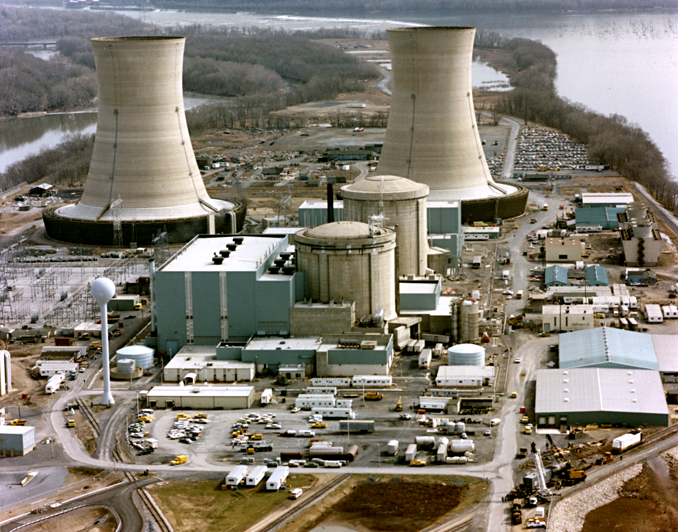
\includegraphics[width=130pt]{images/three-mile-island}}
                {\tiny Source: Wikipedia}
            \end{figure}
        \end{minipage}
        \begin{minipage}[t]{0.58\textwidth}%
            The Three Mile Island Unit 2 (TMI-2) nuclear power plant in Pennsylvania experienced a partial meltdown on
            March 28, 1979 which caused an \alert{increase in radiation level and an explosion within the building},
            there were no casualties.\ The reactor was brought under control after 13.5 hours.
        \end{minipage}

        \framebreak
        Here's a breakdown of what happened:\\[10pt]
        \begin{itemize}
            \small
            \item A malfunction in the demineralizer led to the shutdown of water pumps feeding the reactor core.
            \item Reactor pressure rose, triggering safety measures to insert control rods and stop the fission process.
            \item A pressure relief valve remained open, preventing proper cooling of the reactor core.
            \item Water loss from the core and overheating caused fuel rod damage.
            \item A chemical reaction between steam and reactor components produced hydrogen gas.
        \end{itemize}

        \framebreak

        \textbf{Chernobyl Disaster (\mathbf{1986})}\\[5pt]

        \begin{center}
            \begin{figure}
                \label{fig:chernobyl}
                \copyrightbox[b]
                {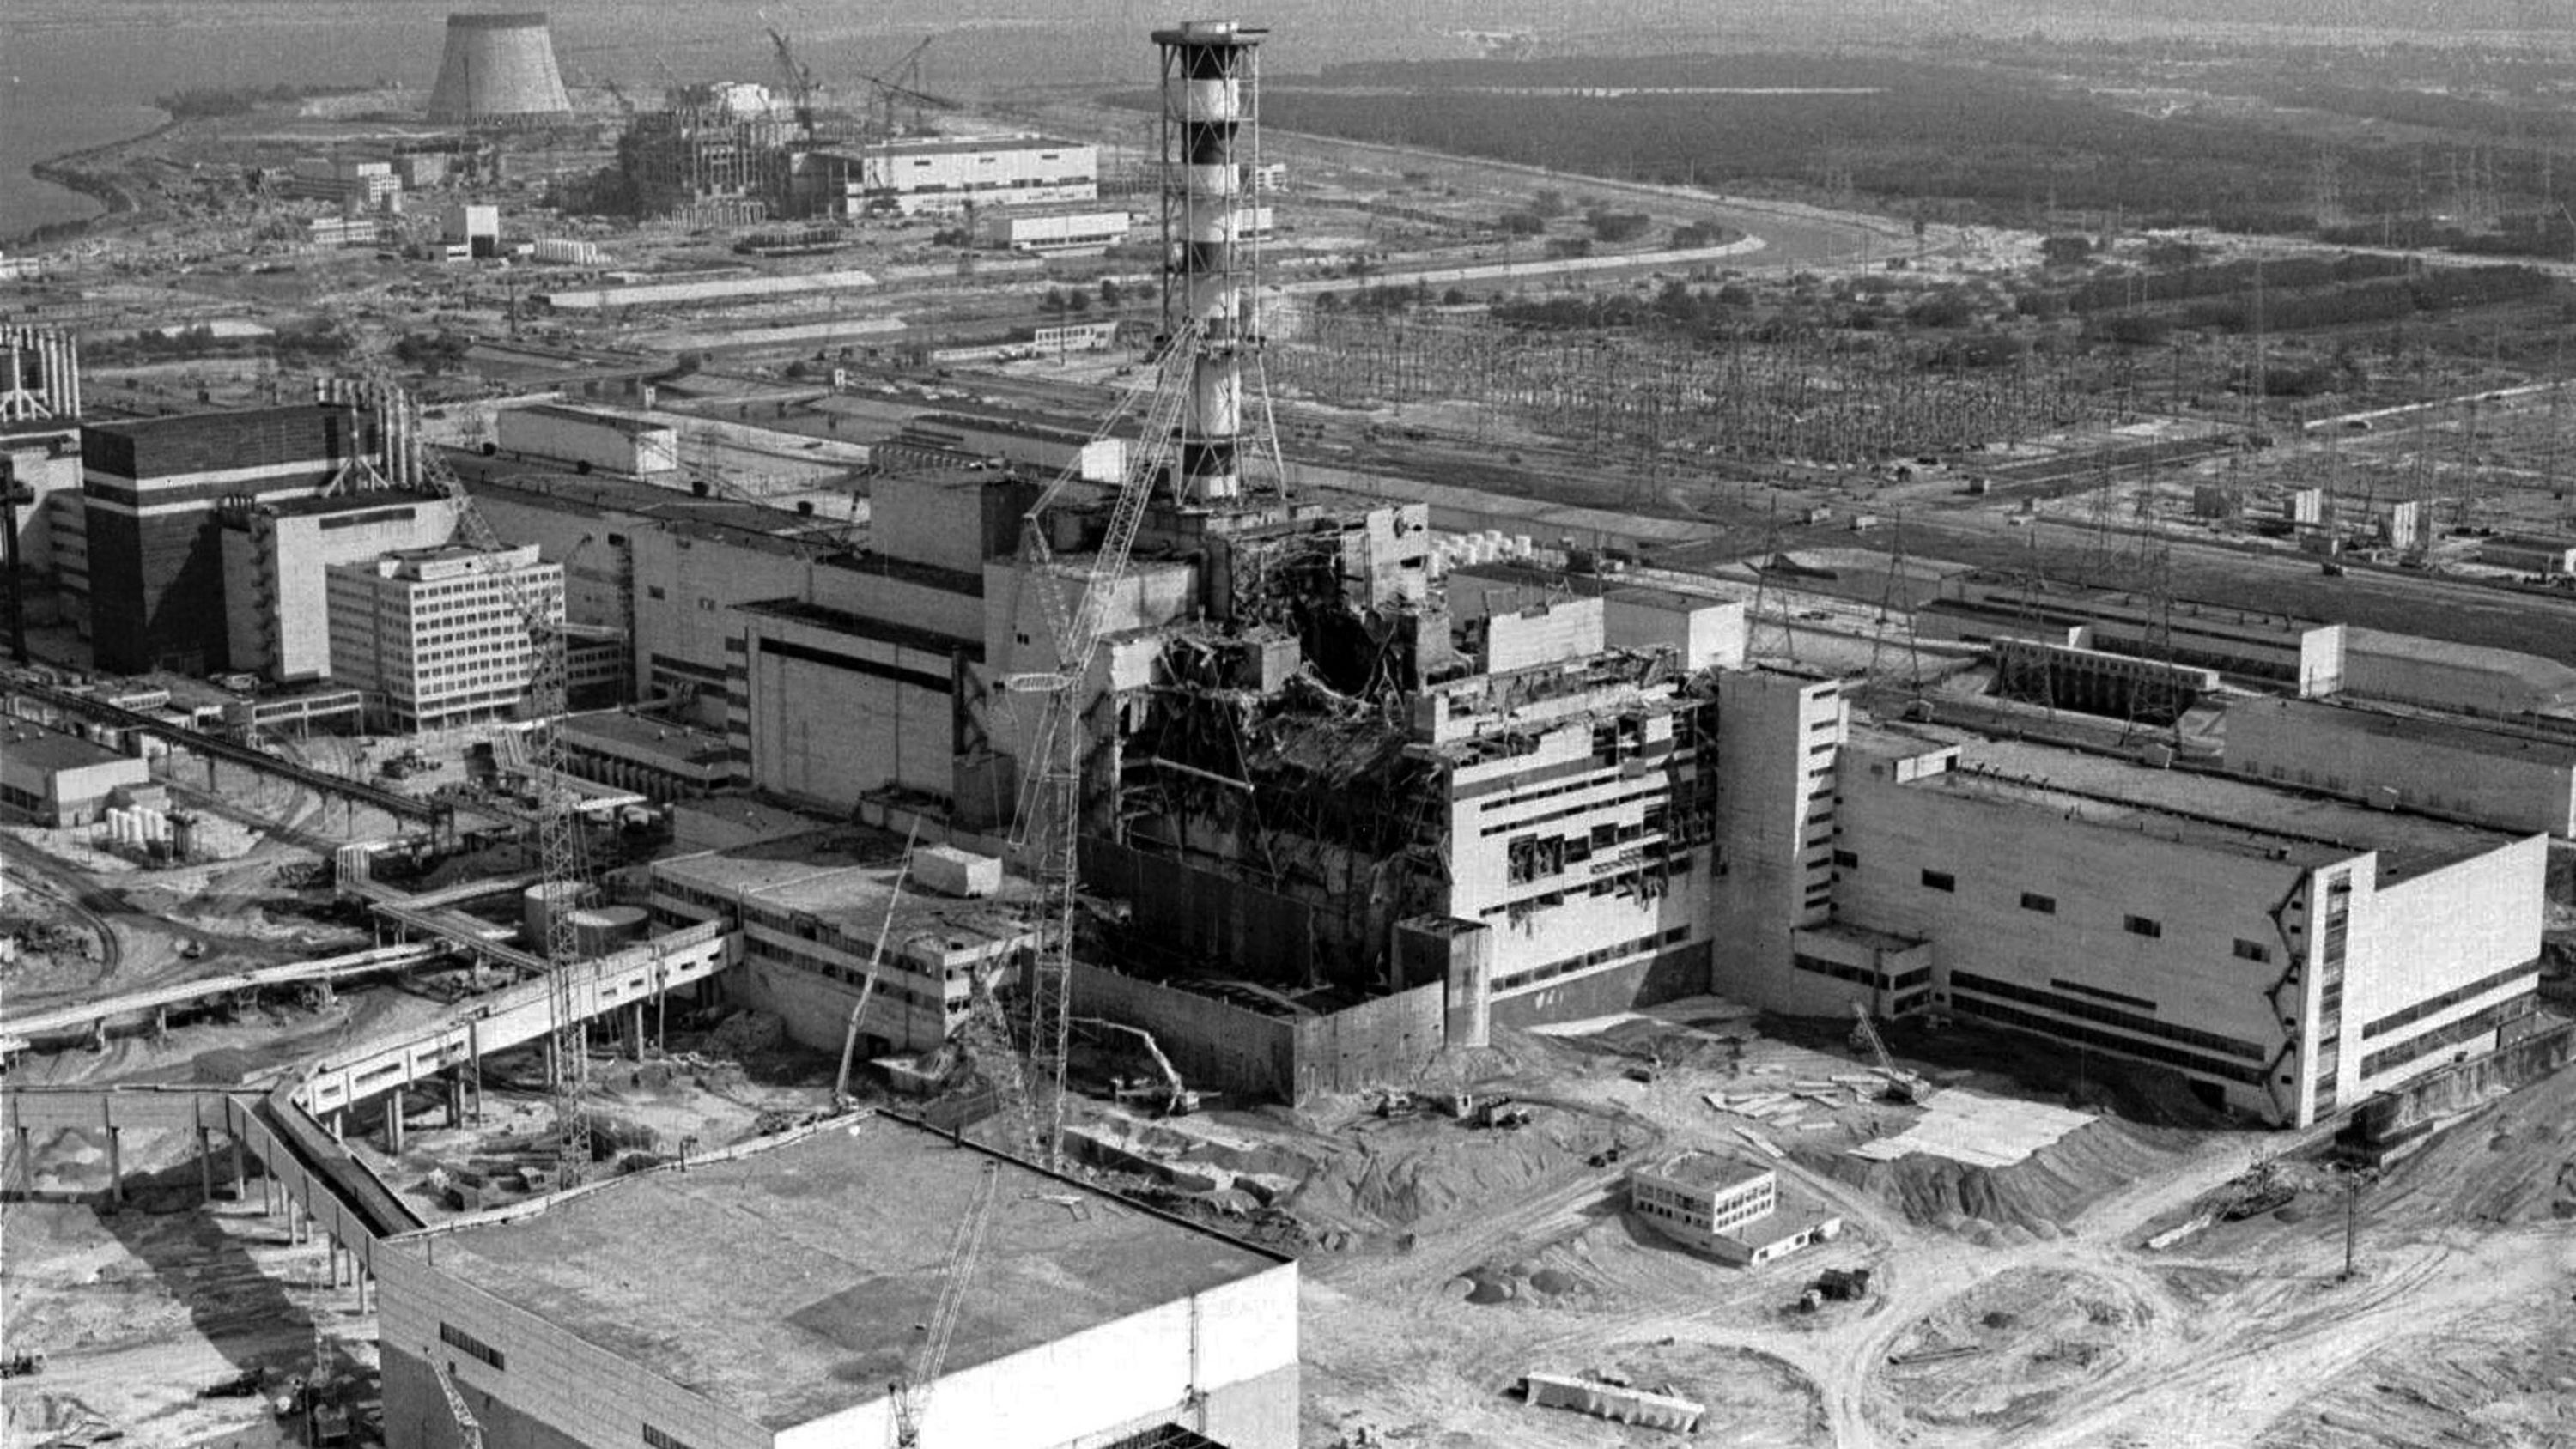
\includegraphics[width=180pt]{images/chernobyl}}
                {\tiny Source: CNN}

            \end{figure}
        \end{center}

        \begin{itemize}
            \item The Chernobyl plant used RBMK reactors, with a graphite water cooling system, known for safety
            vulnerabilities.
            \item A turbine generator test was scheduled during maintenance, requiring a power reduction to 700 MW.
        \end{itemize}

        \begin{itemize}
            \item \textbf{Ignoring Safety Measures:}
            \begin{itemize}
                \item Operators disconnected the emergency cooling system.
                \item The test was conducted at an abnormally low power level (200 MW).
                \item Emergency signals and automatic shutdowns were deliberately blocked.
            \end{itemize}
            \item \textbf{Operator Error and Escalation}
            \begin{itemize}
                \item Operators further compromised safety by raising control rods to increase power, causing a rise
                in reactor temperature and fission rate.
            \end{itemize}
            \item \textbf{Catastrophic Outcome}
            \begin{itemize}
                \item The reactor core melted, leading to a fire and the release of radioactive materials across the
                USSR and Europe.
                \item Evacuation of nearby residents was delayed for hours after the explosion.
            \end{itemize}
            \item \textbf{Casualties and Impact}
            \begin{itemize}
                \item Over 30 plant workers died, with 200 suffering burns.
                \item Long-term health effects resulted in an estimated 8,000 deaths.
                \item Agricultural production was significantly impacted by radioactive contamination for years.
            \end{itemize}
        \end{itemize}
        \\[5pt]
        \textbf{Safety Lessons from TMI and Chernobyl}
        \begin{itemize}
            \item Stronger containment structures to prevent radiation leaks after explosions.
            \item If power increases during critical tests, like at Chernobyl, should be rejected or halted entirely
            with safety systems reactivate
            \item Continuous monitoring of critical components is essential for early detection of issues.
            \item Establish comprehensive emergency plans.
            \item Prompt notification of superiors and timely evacuation of nearby residents (both TMI and Chernobyl).
        \end{itemize}
    \end{frame}

    \begin{frame}[t,allowframebreaks]{Collegiality and Loyalty}
        Craig Ihara defines collegiality as a ``a kind of connectedness grounded in commitment to the goals and
        values of the profession''.\ It is the tendency to support and cooperate with the colleagues.
        \\[5pt]
        \textbf{Elements of Collegiality}\\[5pt]
        \begin{itemize}
            \item \ul{Respect} to the ideas and work of others: This results in support and cooperation with one's
            colleagues.\ One gets back the support and cooperation in return, and this is mutually beneficial.
            \item \ul{Commitment} to moral principles: Commitment is towards moral decisions, actions, goals of
            the organisation and values of the profession.
            \item \ul{Connectedness}: It means the shared commitment and mutual understanding.\ It ensures the
            absense of egoism and paves way for progress in both.
        \end{itemize}

        \framebreak

        \textbf{Loyalty} has two sides:\\[5pt]
        \begin{itemize}
            \item \ul{Agency Loyalty} is about fulfilling your contractual obligations.\ You complete assigned
            tasks and
            cooperate with others.
            \item \ul{Attitude Loyalty} It's about feeling a sense of belonging and wanting to contribute
            positively.\ This loyalty is ideal when the organization works for good.\ However, it shouldn't extend to
            unethical practices.
        \end{itemize}
%
%        \framebreak
%
%        \textbf{Respect for authority} ensures decisions translate to action.\ It comes in two forms:\\[5pt]
%        \begin{itemize}
%            \item \ul{Institutional Authority} is the official power given to managers (like Line Managers) to
%            allocate resources, make decisions, and guide their teams towards achieving goals.
%            \item \ul{Expert Authority} relies on specialized knowledge.\ Experts (consultants, advisors) use
%            their expertise to advise and guide others, not through official power, but through their credibility and
%            proven skills.
%        \end{itemize}
    \end{frame}

    \begin{frame}[t,allowframebreaks]{Collective Bargaining}
        Collective bargaining is a process where trade unions negotiate for better economic benefits for their worker
        members.\ It can involve negotiation, verbal threats, or even strikes.
        \\[10pt]
        \textbf{Ethical Collective Bargaining}\\[5pt]
        \begin{itemize}
            \item Bargaining should be constructive, persuasive, and based on mutual understanding.
            \item Destructive tactics harming people or property are unethical.
        \end{itemize}
        \\[10pt]
        \textbf{Public Interest vs. Worker Interests}\\[5pt]
        \begin{itemize}
            \item A union's actions shouldn't harm the public.\ Strikes by essential workers can threaten public
            safety and health.
            \item Collective bargaining by engineers should consider the public good.
        \end{itemize}

        \framebreak

        \textbf{Professionalism vs. Unionism}\\[5pt]
        There's disagreement about the ethics of union collective bargaining.\\[5pt]
        \begin{itemize}
            \item \textbf{Professional Societies' Perspective:}
            \begin{itemize}
                \item Engineering societies like NSPE believe professional integrity and loyalty to employers come
                first.
                \item See strikes as unprofessional and against the dignity of the profession.
                \item Engineers should act as faithful agents or trustees, putting employer interests before
                self-interest.
            \end{itemize}
            \item \textbf{Considering worker needs:}
            \begin{itemize}
                \item Can engineers be truly loyal if employers ignore worker safety or underpay for extended periods?
                \item Unions can be a necessary tool to ensure fair treatment.
            \end{itemize}
        \end{itemize}
%
%        \framebreak
%
%        \textbf{Unions}\\[5pt]
%        \begin{itemize}
%            \item \textbf{Pros:}
%            \begin{itemize}
%                \item Higher wages \& benefits for workers.
%                \item More worker voice in companies.
%                \item Job security \& protection.
%                \item Fight unethical practices.
%            \end{itemize}
%            \\[5pt]
%            \item \textbf{Cons:}
%            \begin{itemize}
%                \item Inflationary pressures.
%                \item Disruptions \& lost productivity.
%                \item Discourages merit-based rewards.
%                \item May worsen labour relations.
%                \item Limits job flexibility.
%            \end{itemize}
%        \end{itemize}
    \end{frame}

    \begin{frame}[t,allowframebreaks]{Confidentiality}
        \textbf{Confidentiality} is about keeping information about employers and clients secret, and is a
        cornerstone of ethical teamwork.
        \\[10pt]
        \textbf{Importance}\\[5pt]
        Several ethical theories justify confidentiality:\\[5pt]
        \begin{itemize}
            \item \ul{Rights and Duties:} It protects stakeholders' rights, like a company's intellectual
            property, and upholds the mutual trust between employers and employees.
            \item \ul{Utilitarianism:} creates the most good for the most people.
        \end{itemize}

        \framebreak

        \textbf{Moral Principles}\\[5pt]
        Confidentiality is supported by these moral principles:\\[5pt]
        \begin{itemize}
            \item \ul{Respect for Autonomy:} Individuals and organizations have the right to control their
            information.
            \item \ul{Respect for Promises:} Employees honour agreements with employers regarding sensitive
            information.
            \item \ul{Trustworthiness:} Maintaining confidentiality is essential in professions like law and
            medicine, fostering trust and open communication.
            \item \ul{Respect for Public Welfare:} When used ethically, confidentiality benefits the public.\ For
            example, doctor-patient confidentiality encourages patients to seek help, leading to better healthcare.
        \end{itemize}

        \framebreak

        \textbf{Confidential Information: Types and Challenges}\\[10pt]
        \textbf{Types of Confidential Information:}\\[5pt]
        \begin{itemize}
            \item \ul{Privileged Information:} Information accessed due to job assignment, like details about a
            defence project.
            \item \ul{Proprietary Information:} Knowledge and procedures owned by the organization, protected legally
            like trade secrets, quality manuals etc.
        \end{itemize}
        \textbf{Confidentiality by Severity:}\\[5pt]
        \begin{itemize}
            \item \ul{Obvious Information:} Highly sensitive data related to unreleased products, designs, formulas,
            or technical processes.\ Leaking this could threaten the company's survival.
            \item \ul{Less Confidential Information:} Business details like employee numbers, supplier identities,
            marketing strategies, or manufacturing costs.
        \end{itemize}
        \textbf{Switching Jobs and Confidentiality:}
        \begin{itemize}
            \small
            \item \textbf{Arguments for Maintaining Confidentiality:}
            \begin{itemize}
                \item Employee integrity and professional ethics demand protecting confidential information even
                after leaving a job.
            \end{itemize}
            \item \textbf{Counterarguments:}
            \begin{itemize}
                \item Employees' expertise and knowledge are valuable assets they bring to a new role.
                \item Courts have balanced employer rights with employee rights to career advancement.
            \end{itemize}
        \end{itemize}
        \textbf{Management Strategies (with Limitations):}
        \begin{itemize}
            \small
            \item Contracts limiting future employment geographically, by time gap, or by type of job (not legally
            enforceable everywhere).
            \item Offering financial compensation in exchange for restricting future job options.
            \item Limiting access to sensitive information can hinder creativity and innovation.
        \end{itemize}
    \end{frame}

    \begin{frame}[t,allowframebreaks]{Conflict of Interest}
        A conflict of interest arises when an employee has multiple interests that could potentially clash, which might
        hinder their ability to fulfill their obligations to their employer or client.\\[10pt]
        \begin{minipage}[t]{0.6\textwidth}
            \small
            \textbf{Types of Conflicts of Interest:}
            \begin{itemize}
                \item \ul{Actual Conflict:} Objectivity is compromised due to outside interests, leading to an inability
                to fulfil one's professional duties.
                \item \ul{Apparent Conflict:} Creates the impression that professional judgment is compromised.
                \item \ul{Potential Conflict:} Involves the interests of an employee's spouse, relative, or friend,
                potentially influencing their judgment in favor of the outsider.
            \end{itemize}
        \end{minipage}
        \begin{minipage}[t]{0.05\textwidth}
            ~
        \end{minipage}
        \begin{minipage}[t]{0.3\textwidth}
            \small
            \vspace*{-8pt}
            \begin{block}{Distinguishing from Conflicting Interests:}
                \footnotesize
                Imagine a student struggling to study for four exams but only having time for three.\ This is a
                situation of conflicting interests, not a moral dilemma.
            \end{block}
        \end{minipage}

        \framebreak

        \textbf{Favorable Contract:}
        A conflict arises when an engineer has the power to award contracts (subcontracts, purchase orders) to a
        company where their spouse or they themselves have a financial interest (stock-holding).
        \\[10pt]

        \textbf{Bribery vs. Gifts}\\[5pt]
        \begin{tblr}{colspec=|X|X|X|,hlines,cells={font=\fontsize{8pt}\selectfont}}
            \textbf{Feature}                 & \textbf{Bribe}       & \textbf{Gift}            \\
            \textbf{Timing}                  & Before a decision    & After a decision         \\
            \textbf{Cost}                    & Large Amount         & Small amount             \\
            \textbf{Quality}                 & Poor                 & Good/High                \\
            \textbf{Giver's Relationship}    & Friend               & Not necessarily a friend \\
            \textbf{Transparency}            & Secret               & Open                     \\
            \textbf{Motive}                  & Undue favor expected & Favor or gratitude       \\
            \textbf{Consequence on Employer} & Damages reputation   & No damage                \\
        \end{tblr}

        \framebreak

        \textbf{Company policies on gifts:}\\[5pt]
        While codes of ethics generally discourage gifts, some companies may have flexible policies
        allowing small tokens.\ Gifts should not influence professional judgment.
        \\[10pt]
        \textbf{Moonlighting:}\\[5pt]
        Working for two companies if:
        \begin{itemize}
            \small
            \item The companies are competitors, suppliers, or customers of your primary employer.
            \item It leads to exhaustion and harms your performance in both jobs.
        \end{itemize}
        \\[10pt]
        \textbf{Insider Information:}\\[5pt]
        Using confidential information from your employer, client, or business partner.\ Examples include trading
        stocks based on knowledge of mergers, acquisitions, or new strategies.
    \end{frame}

    \begin{frame}{End}
        \begin{center}
            \huge The End.
        \end{center}
    \end{frame}
\end{document}